
%% bare_conf.tex
%% V1.3
%% 2007/01/11
%% by Michael Shell
%% See:
%% http://www.michaelshell.org/
%% for current contact information.
%%
%% This is a skeleton file demonstrating the use of IEEEtran.cls
%% (requires IEEEtran.cls version 1.7 or later) with an IEEE conference paper.
%%
%% Support sites:
%% http://www.michaelshell.org/tex/ieeetran/
%% http://www.ctan.org/tex-archive/macros/latex/contrib/IEEEtran/
%% and
%% http://www.ieee.org/

%%*************************************************************************
%% Legal Notice:
%% This code is offered as-is without any warranty either expressed or
%% implied; without even the implied warranty of MERCHANTABILITY or
%% FITNESS FOR A PARTICULAR PURPOSE!
%% User assumes all risk.
%% In no event shall IEEE or any contributor to this code be liable for
%% any damages or losses, including, but not limited to, incidental,
%% consequential, or any other damages, resulting from the use or misuse
%% of any information contained here.
%%
%% All comments are the opinions of their respective authors and are not
%% necessarily endorsed by the IEEE.
%%
%% This work is distributed under the LaTeX Project Public License (LPPL)
%% ( http://www.latex-project.org/ ) version 1.3, and may be freely used,
%% distributed and modified. A copy of the LPPL, version 1.3, is included
%% in the base LaTeX documentation of all distributions of LaTeX released
%% 2003/12/01 or later.
%% Retain all contribution notices and credits.
%% ** Modified files should be clearly indicated as such, including  **
%% ** renaming them and changing author support contact information. **
%%
%% File list of work: IEEEtran.cls, IEEEtran_HOWTO.pdf, bare_adv.tex,
%%                    bare_conf.tex, bare_jrnl.tex, bare_jrnl_compsoc.tex
%%*************************************************************************

% *** Authors should verify (and, if needed, correct) their LaTeX system  ***
% *** with the testflow diagnostic prior to trusting their LaTeX platform ***
% *** with production work. IEEE's font choices can trigger bugs that do  ***
% *** not appear when using other class files.                            ***
% The testflow support page is at:
% http://www.michaelshell.org/tex/testflow/



% Note that the a4paper option is mainly intended so that authors in
% countries using A4 can easily print to A4 and see how their papers will
% look in print - the typesetting of the document will not typically be
% affected with changes in paper size (but the bottom and side margins will).
% Use the testflow package mentioned above to verify correct handling of
% both paper sizes by the user's LaTeX system.
%
% Also note that the "draftcls" or "draftclsnofoot", not "draft", option
% should be used if it is desired that the figures are to be displayed in
% draft mode.
%
\documentclass[conference]{IEEEtran}
% Add the compsoc option for Computer Society conferences.
%
% If IEEEtran.cls has not been installed into the LaTeX system files,
% manually specify the path to it like:
% \documentclass[conference]{../sty/IEEEtran}


\IEEEoverridecommandlockouts %To add sponsors and index terms


% Some very useful LaTeX packages include:
% (uncomment the ones you want to load)


% *** MISC UTILITY PACKAGES ***
%
%\usepackage{ifpdf}
% Heiko Oberdiek's ifpdf.sty is very useful if you need conditional
% compilation based on whether the output is pdf or dvi.
% usage:
% \ifpdf
%   % pdf code
% \else
%   % dvi code
% \fi
% The latest version of ifpdf.sty can be obtained from:
% http://www.ctan.org/tex-archive/macros/latex/contrib/oberdiek/
% Also, note that IEEEtran.cls V1.7 and later provides a builtin
% \ifCLASSINFOpdf conditional that works the same way.
% When switching from latex to pdflatex and vice-versa, the compiler may
% have to be run twice to clear warning/error messages.






% *** CITATION PACKAGES ***
%
\usepackage{cite}
% cite.sty was written by Donald Arseneau
% V1.6 and later of IEEEtran pre-defines the format of the cite.sty package
% \cite{} output to follow that of IEEE. Loading the cite package will
% result in citation numbers being automatically sorted and properly
% "compressed/ranged". e.g., [1], [9], [2], [7], [5], [6] without using
% cite.sty will become [1], [2], [5]--[7], [9] using cite.sty. cite.sty's
% \cite will automatically add leading space, if needed. Use cite.sty's
% noadjust option (cite.sty V3.8 and later) if you want to turn this off.
% cite.sty is already installed on most LaTeX systems. Be sure and use
% version 4.0 (2003-05-27) and later if using hyperref.sty. cite.sty does
% not currently provide for hyperlinked citations.
% The latest version can be obtained at:
% http://www.ctan.org/tex-archive/macros/latex/contrib/cite/
% The documentation is contained in the cite.sty file itself.






% *** GRAPHICS RELATED PACKAGES ***
%
\ifCLASSINFOpdf
   \usepackage[pdftex]{graphicx}
  % declare the path(s) where your graphic files are
   \graphicspath{{./Images/}}
  % and their extensions so you won't have to specify these with
  % every instance of \includegraphics
   \DeclareGraphicsExtensions{.pdf,.jpeg,.png}
\else
  % or other class option (dvipsone, dvipdf, if not using dvips). graphicx
  % will default to the driver specified in the system graphics.cfg if no
  % driver is specified.
  % \usepackage[dvips]{graphicx}
  % declare the path(s) where your graphic files are
  % \graphicspath{{../eps/}}
  % and their extensions so you won't have to specify these with
  % every instance of \includegraphics
  % \DeclareGraphicsExtensions{.eps}
\fi
% graphicx was written by David Carlisle and Sebastian Rahtz. It is
% required if you want graphics, photos, etc. graphicx.sty is already
% installed on most LaTeX systems. The latest version and documentation can
% be obtained at:
% http://www.ctan.org/tex-archive/macros/latex/required/graphics/
% Another good source of documentation is "Using Imported Graphics in
% LaTeX2e" by Keith Reckdahl which can be found as epslatex.ps or
% epslatex.pdf at: http://www.ctan.org/tex-archive/info/
%
% latex, and pdflatex in dvi mode, support graphics in encapsulated
% postscript (.eps) format. pdflatex in pdf mode supports graphics
% in .pdf, .jpeg, .png and .mps (metapost) formats. Users should ensure
% that all non-photo figures use a vector format (.eps, .pdf, .mps) and
% not a bitmapped formats (.jpeg, .png). IEEE frowns on bitmapped formats
% which can result in "jaggedy"/blurry rendering of lines and letters as
% well as large increases in file sizes.
%
% You can find documentation about the pdfTeX application at:
% http://www.tug.org/applications/pdftex





% *** MATH PACKAGES ***
%
\usepackage[cmex10]{amsmath}
% A popular package from the American Mathematical Society that provides
% many useful and powerful commands for dealing with mathematics. If using
% it, be sure to load this package with the cmex10 option to ensure that
% only type 1 fonts will utilized at all point sizes. Without this option,
% it is possible that some math symbols, particularly those within
% footnotes, will be rendered in bitmap form which will result in a
% document that can not be IEEE Xplore compliant!
%
% Also, note that the amsmath package sets \interdisplaylinepenalty to 10000
% thus preventing page breaks from occurring within multiline equations. Use:
%\interdisplaylinepenalty=2500
% after loading amsmath to restore such page breaks as IEEEtran.cls normally
% does. amsmath.sty is already installed on most LaTeX systems. The latest
% version and documentation can be obtained at:
% http://www.ctan.org/tex-archive/macros/latex/required/amslatex/math/





% *** SPECIALIZED LIST PACKAGES ***
%
%\usepackage{algorithmic}
% algorithmic.sty was written by Peter Williams and Rogerio Brito.
% This package provides an algorithmic environment fo describing algorithms.
% You can use the algorithmic environment in-text or within a figure
% environment to provide for a floating algorithm. Do NOT use the algorithm
% floating environment provided by algorithm.sty (by the same authors) or
% algorithm2e.sty (by Christophe Fiorio) as IEEE does not use dedicated
% algorithm float types and packages that provide these will not provide
% correct IEEE style captions. The latest version and documentation of
% algorithmic.sty can be obtained at:
% http://www.ctan.org/tex-archive/macros/latex/contrib/algorithms/
% There is also a support site at:
% http://algorithms.berlios.de/index.html
% Also of interest may be the (relatively newer and more customizable)
% algorithmicx.sty package by Szasz Janos:
% http://www.ctan.org/tex-archive/macros/latex/contrib/algorithmicx/




% *** ALIGNMENT PACKAGES ***
%
%\usepackage{array}
% Frank Mittelbach's and David Carlisle's array.sty patches and improves
% the standard LaTeX2e array and tabular environments to provide better
% appearance and additional user controls. As the default LaTeX2e table
% generation code is lacking to the point of almost being broken with
% respect to the quality of the end results, all users are strongly
% advised to use an enhanced (at the very least that provided by array.sty)
% set of table tools. array.sty is already installed on most systems. The
% latest version and documentation can be obtained at:
% http://www.ctan.org/tex-archive/macros/latex/required/tools/


%\usepackage{mdwmath}
%\usepackage{mdwtab}
% Also highly recommended is Mark Wooding's extremely powerful MDW tools,
% especially mdwmath.sty and mdwtab.sty which are used to format equations
% and tables, respectively. The MDWtools set is already installed on most
% LaTeX systems. The lastest version and documentation is available at:
% http://www.ctan.org/tex-archive/macros/latex/contrib/mdwtools/


% IEEEtran contains the IEEEeqnarray family of commands that can be used to
% generate multiline equations as well as matrices, tables, etc., of high
% quality.


%\usepackage{eqparbox}
% Also of notable interest is Scott Pakin's eqparbox package for creating
% (automatically sized) equal width boxes - aka "natural width parboxes".
% Available at:
% http://www.ctan.org/tex-archive/macros/latex/contrib/eqparbox/





% *** SUBFIGURE PACKAGES ***
%\usepackage[tight,footnotesize]{subfigure}
% subfigure.sty was written by Steven Douglas Cochran. This package makes it
% easy to put subfigures in your figures. e.g., "Figure 1a and 1b". For IEEE
% work, it is a good idea to load it with the tight package option to reduce
% the amount of white space around the subfigures. subfigure.sty is already
% installed on most LaTeX systems. The latest version and documentation can
% be obtained at:
% http://www.ctan.org/tex-archive/obsolete/macros/latex/contrib/subfigure/
% subfigure.sty has been superceeded by subfig.sty.



%\usepackage[caption=false]{caption}
%\usepackage[font=footnotesize]{subfig}
% subfig.sty, also written by Steven Douglas Cochran, is the modern
% replacement for subfigure.sty. However, subfig.sty requires and
% automatically loads Axel Sommerfeldt's caption.sty which will override
% IEEEtran.cls handling of captions and this will result in nonIEEE style
% figure/table captions. To prevent this problem, be sure and preload
% caption.sty with its "caption=false" package option. This is will preserve
% IEEEtran.cls handing of captions. Version 1.3 (2005/06/28) and later
% (recommended due to many improvements over 1.2) of subfig.sty supports
% the caption=false option directly:
%\usepackage[caption=false,font=footnotesize]{subfig}
%
% The latest version and documentation can be obtained at:
% http://www.ctan.org/tex-archive/macros/latex/contrib/subfig/
% The latest version and documentation of caption.sty can be obtained at:
% http://www.ctan.org/tex-archive/macros/latex/contrib/caption/




% *** FLOAT PACKAGES ***
%
%\usepackage{fixltx2e}
% fixltx2e, the successor to the earlier fix2col.sty, was written by
% Frank Mittelbach and David Carlisle. This package corrects a few problems
% in the LaTeX2e kernel, the most notable of which is that in current
% LaTeX2e releases, the ordering of single and double column floats is not
% guaranteed to be preserved. Thus, an unpatched LaTeX2e can allow a
% single column figure to be placed prior to an earlier double column
% figure. The latest version and documentation can be found at:
% http://www.ctan.org/tex-archive/macros/latex/base/



%\usepackage{stfloats}
% stfloats.sty was written by Sigitas Tolusis. This package gives LaTeX2e
% the ability to do double column floats at the bottom of the page as well
% as the top. (e.g., "\begin{figure*}[!b]" is not normally possible in
% LaTeX2e). It also provides a command:
%\fnbelowfloat
% to enable the placement of footnotes below bottom floats (the standard
% LaTeX2e kernel puts them above bottom floats). This is an invasive package
% which rewrites many portions of the LaTeX2e float routines. It may not work
% with other packages that modify the LaTeX2e float routines. The latest
% version and documentation can be obtained at:
% http://www.ctan.org/tex-archive/macros/latex/contrib/sttools/
% Documentation is contained in the stfloats.sty comments as well as in the
% presfull.pdf file. Do not use the stfloats baselinefloat ability as IEEE
% does not allow \baselineskip to stretch. Authors submitting work to the
% IEEE should note that IEEE rarely uses double column equations and
% that authors should try to avoid such use. Do not be tempted to use the
% cuted.sty or midfloat.sty packages (also by Sigitas Tolusis) as IEEE does
% not format its papers in such ways.





% *** PDF, URL AND HYPERLINK PACKAGES ***
%
%\usepackage{url}
% url.sty was written by Donald Arseneau. It provides better support for
% handling and breaking URLs. url.sty is already installed on most LaTeX
% systems. The latest version can be obtained at:
% http://www.ctan.org/tex-archive/macros/latex/contrib/misc/
% Read the url.sty source comments for usage information. Basically,
% \url{my_url_here}.





% *** Do not adjust lengths that control margins, column widths, etc. ***
% *** Do not use packages that alter fonts (such as pslatex).         ***
% There should be no need to do such things with IEEEtran.cls V1.6 and later.
% (Unless specifically asked to do so by the journal or conference you plan
% to submit to, of course. )

\usepackage[hidelinks]{hyperref}
%for columns spanning multiple rows in tables
\usepackage{multirow}
%use the booktabs package to get (much!) better vertical spacing above and below "rules" (horizontal lines), resulting in a much more professional look of your tables.
%use the colortbl package to add color to tables.
\usepackage{booktabs,colortbl}

% correct bad hyphenation here
\hyphenation{op-tical net-works semi-conduc-tor}

  \renewcommand\footnoterule{\vspace*{-3pt}%
     \hrule width 2in height 0.4pt
     \vspace*{2.6pt}}

\begin{document}
%
% paper title
% can use linebreaks \\ within to get better formatting as desired
\title{Preparation of a Paper for the\\
IEEE PowerTech 2015 Conference}


% author names and affiliations
% use a multiple column layout for up to two different
% affiliations
\author{%

\IEEEauthorblockN{Line 1: Author Name/s per 1st Affiliation \\ Line 2: Author Name/s per 1st Affiliation }
\IEEEauthorblockA{Line 3 (of \emph{Affiliation}): Dept. name of organization\\
Line 4: name of organization, acronyms acceptable\\
Line 5: City, Country\\
Line 6: e-mail address, if desired}
\and
\IEEEauthorblockN{Line 1: Author Name/s per 2nd Affiliation \\ Line 2: Author Name/s per 2nd Affiliation }
\IEEEauthorblockA{Line 3 (of \emph{Affiliation}): Dept. name of organization\\
Line 4: name of organization, acronyms acceptable\\
Line 5: City, Country\\
Line 6: e-mail address, if desired}

% use \thanks{} to gain access to the first footnote area
% a separate \thanks must be used for each paragraph as LaTeX2e's \thanks
% was not built to handle multiple paragraphs
%

\thanks{Identify applicable sponsor/s here. \emph{(sponsors)}}%

}

% use for special paper notices
%\IEEEspecialpapernotice{(Invited Paper)}


% make the title area
\maketitle

%ABSTRACT
\begin{abstract}
Basic guidelines for the preparation of an extended abstract and/or full paper for the PowerTech 2015 Conference are presented. This \LaTeX{} document is a ``live'' template. The various components of your paper [title, text, headings, etc.] are already defined in the IEEEtran document class, as illustrated by the portions given in this document. The abstract is limited to 150 words and cannot contain equations, figures, tables, or references. It should concisely state what was done, how it was done, principal results, and their significance.\\
\end{abstract}

%INDEX TERMS
\begin{IEEEkeywords}
The author shall provide up to 4 keywords (in alphabetical order) to help identify the major topics of the paper. The thesaurus of IEEE indexing keywords is posted at \linebreak \url{http://www.ieee.org/organizations/pubs/ani_prod/keywrd98.txt}.
\end{IEEEkeywords}


\section{Introduction}

This template provides authors with most of the formatting specifications needed for preparing electronic versions of PowerTech 2015 Conference papers based on the IEEE PES Author's Kit. All standard paper components have been specified for three reasons: (1) ease of use when formatting individual papers, (2) automatic compliance to electronic requirements that facilitate the concurrent or later production of electronic products, and (3) conformity of style throughout a conference’s proceedings. Margins, column widths, line spacing, and type styles are built-in; examples of the type styles are provided throughout this document and are identified in italic type, within parentheses, following the example. Some components, such as multi-leveled equations, graphics, and tables are not prescribed, although the various table text styles are provided. The formatter will need to create these components, incorporating the applicable criteria that follow.

\section{Ease of Use}

\subsection{Template}
This template has been tailored for output on US letter-sized paper.

\subsection{Maintaining the Integrity of the Specifications}
The template is used to format your paper and style the text. All margins, column widths, line spaces, and text fonts are prescribed; please do not alter them. You may note peculiarities. For example, the heading margin in this template measures proportionately more than is customary. This measurement and others are deliberate, using specifications that anticipate your paper as one part of the entire proceedings, and not as an independent document. Please do not revise any of the current designations.

\section{Extended Abstract/Full Paper Preparation}
Extended abstracts should be two to three pages long. Full papers are limited to a maximum of six pages. Please use automatic hyphenation and check your spelling. Additionally, be sure your sentences are complete and that there is continuity within your paragraphs. Make sure that all appropriate references are included. \LaTeX{} will sort the section, figure, equation, and table numbers automatically.

Please take note of the following items when proofreading spelling and grammar:

\subsection{Abbreviations and Acronyms}
Define abbreviations and acronyms the first time they are used in the text, even after they have been defined in the abstract. Abbreviations such as IEEE, SI, ac, dc, and rms do not have to be defined. Do not use abbreviations in the title or section headings unless they are unavoidable.

\subsection{Units}
\begin{itemize}
    \item Metric units are preferred for use in IEEE publications in light of their global readership and the inherent convenience of these units in many fields. In particular, the use of the International System of Units (\emph{Systeme Internationale d'Unit\'{e}s} or SI Units) is advocated. This system includes a subsystem of units based on the meter, kilogram, second, and ampere (MKSA). U.S. Customary units, or British units, may be used as secondary units (in parentheses). An exception is when U.S. Customary units are used as identifiers in trade, such as 3.5-inch disk drive.

    \item Avoid combining SI and U.S. Customary units, such as current in amperes and magnetic field in oersteds. This often leads to confusion because equations do not balance dimensionally. If you must use mixed units, clearly state the units for each quantity that you use in an equation.

    \item Do not mix complete spellings and abbreviations of units: ``Wb/m2'' or ``webers per square meter'', not ``webers/m2''.  Spell out units when they appear in text: ``\ldots a few henries", not ``\ldots a few H".

    \item Use a zero before decimal points: ``0.25", not ``.25". Use ``cm3", not ``cc". \emph{(bullet list)}
\end{itemize}

\subsection{Equations}
Equations are created using the \texttt{equation} environment. To create multileveled equations, use the \texttt{amsmath} extension package for \LaTeX{}. To make your equations more compact, you may use the solidus ( / ), the exp function, or appropriate exponents. Punctuate equations with commas or periods when they are part of a sentence, as in
\begin{equation}
\label{eqn:example}
\alpha - \beta + \delta = \chi.
\end{equation}

Be sure that the symbols in your equation have been defined before or immediately following the equation. Use ``(\ref{eqn:example})", not ``Eq. (\ref{eqn:example})" or ``equation (\ref{eqn:example})", except at the beginning of a sentence: ``Equation (\ref{eqn:example}) is \ldots"

\subsection{Footnotes}
Create footnotes with the \texttt{footnote} environment. Do not put footnotes in the reference list. Use letters for table footnotes, as shown in Table \ref{tab:example}.

\subsection{Some Common Mistakes}
\begin{itemize}

    \item The word ``data" is plural, not singular.

    \item The subscript for the permeability of vacuum $\mu_0$, and other common scientific constants, is zero with subscript formatting, not a lowercase letter ``o".

    \item In American English, commas, semi-/colons, periods, question and exclamation marks are located within quotation marks only when a complete thought or name is cited, such as a title or full quotation. When quotation marks are used, instead of a bold or italic typeface, to highlight a word or phrase, punctuation should appear outside of the quotation marks. A parenthetical phrase or statement at the end of a sentence is punctuated outside of the closing parenthesis (like this). (A parenthetical sentence is punctuated within the parentheses.)

    \item A graph within a graph is an ``inset", not an ``insert". The word alternatively is preferred to the word ``alternately" (unless you really mean something that alternates).

    \item Do not use the word ``essentially" to mean ``approximately" or ``effectively".

    \item In your paper title, if the words ``that uses" can accurately replace the word ``using", capitalize the ``u"; if not, keep using lower-cased.

    \item Be aware of the different meanings of the homophones ``affect" and ``effect", ``complement" and "compliment", ``discreet" and ``discrete", ``principal" and ``principle".

    \item Do not confuse ``imply" and ``infer".

    \item The prefix ``non" is not a word; it should be joined to the word it modifies, usually without a hyphen.

    \item There is no period after the ``et" in the Latin abbreviation ``et al.".

    \item The abbreviation ``i.e." means ``that is", and the abbreviation ``e.g." means ``for example".

\end{itemize}

\section{Using the Template}
This document should be used as a template for preparing your Extended Abstract and Full Conference Paper. You may type over sections of the document, cut and paste into it, and/or use markup styles.

Duplicate the template file by using the Save As command, and use the naming convention prescribed by your conference for the name of your paper.

\subsection{Authors and Affiliations}
The template is designed so that author affiliations are not repeated each time for multiple authors of the same affiliation. Please keep your affiliations as succinct as possible (for example, do not differentiate among departments of the same organization). This template was designed for two affiliations.

\subsection{Identify the Headings}
Headings are organizational devices that guide the reader through your paper. There are two types: component headings and text headings.

Component headings identify the different components of your paper and are not topically subordinate to each other. Examples include \textsc{Acknowledgments} and \textsc{References} and, for these, it is necessary to use the \texttt{\textbackslash section} command. Use \texttt{\textbackslash caption} within the table and figure environments for your figure captions and table titles.

Text headings organize the topics on a relational, hierarchical basis. For example, the paper title is the primary text heading because all subsequent material relates and elaborates on this one topic. If there are two or more sub-topics, the next level heading should be used and, conversely, if there are not at least two sub-topics, then no subheadings should be introduced. The sectioning commands \texttt{\textbackslash subsection}, \texttt{\textbackslash subsubsection}, and \texttt{\textbackslash paragraph} are prescribed.

\subsection{Figures and Tables}
\subsubsection{Positioning Figures and Tables}

Large figures and tables may span across both columns. Figure captions should be below the figures; table headings should appear above the tables. Insert figures and tables after they are cited in the text as close to the citation as possible. Use the abbreviation ``Fig. \ref{fig:example}", even at the beginning of a sentence.

% An example of a floating table. Note that, for IEEE style tables, the
% \caption command should come BEFORE the table. Table text will default to
% \footnotesize as IEEE normally uses this smaller font for tables.
% The \label must come after \caption as always.

\begin{table}[!ht]
%% increase table row spacing, adjust to taste
\renewcommand{\arraystretch}{1.2}
%% if using array.sty, it might be a good idea to tweak the value of
%% \extrarowheight as needed to properly center the text within the cells
%
\caption{Table Type Styles}
\label{tab:example}
\noindent
\centering
    \begin{minipage}{\linewidth} %Use the minipage environment to footnote tables
    \renewcommand\footnoterule{\vspace*{-5pt}} %to remove the horizontal rule above the table footnote
    \begin{center}
        \begin{tabular}{c c c c}
            \toprule
            \multirow{2}{*}{Table Heading} & \multicolumn{3}{c}{Table Column Heading} \\
            \cline{2-4}
             & Table column subheading & Subheading & Subheading \\
            \midrule
            Copy & More table copy \footnote{Example of a table footnote.} & &\\
            \bottomrule
        \end{tabular}
        \end{center}
    \end{minipage}
\end{table}

\subsubsection{Figure Labels}
Use words rather than symbols or abbreviations when writing Figure axis labels to avoid confusing the reader. As an example, write the quantity ``Magnetization", or ``Magnetization, M", not just ``M". If including units in the label, present them within parentheses. Do not label axes only with units. In the example, write ``Magnetization (A/m)" or ``Magnetization {A[m(1)]}", not just ``A/m". Do not label axes with a ratio of quantities and units. For example, write ``Temperature (K)", not ``Temperature/K”.
Figures and tables should be numbered consecutively.

% An example of a floating figure using the graphicx package.
% Note that \label must occur AFTER (or within) \caption.
% For figures, \caption should occur after the \includegraphics.
% Note that IEEEtran v1.7 and later has special internal code that
% is designed to preserve the operation of \label within \caption
% even when the captionsoff option is in effect. However, because
% of issues like this, it may be the safest practice to put all your
% \label just after \caption rather than within \caption{}.
%
% Reminder: the "draftcls" or "draftclsnofoot", not "draft", class
% option should be used if it is desired that the figures are to be
% displayed while in draft mode.
%
\begin{figure}[!ht]
\centering
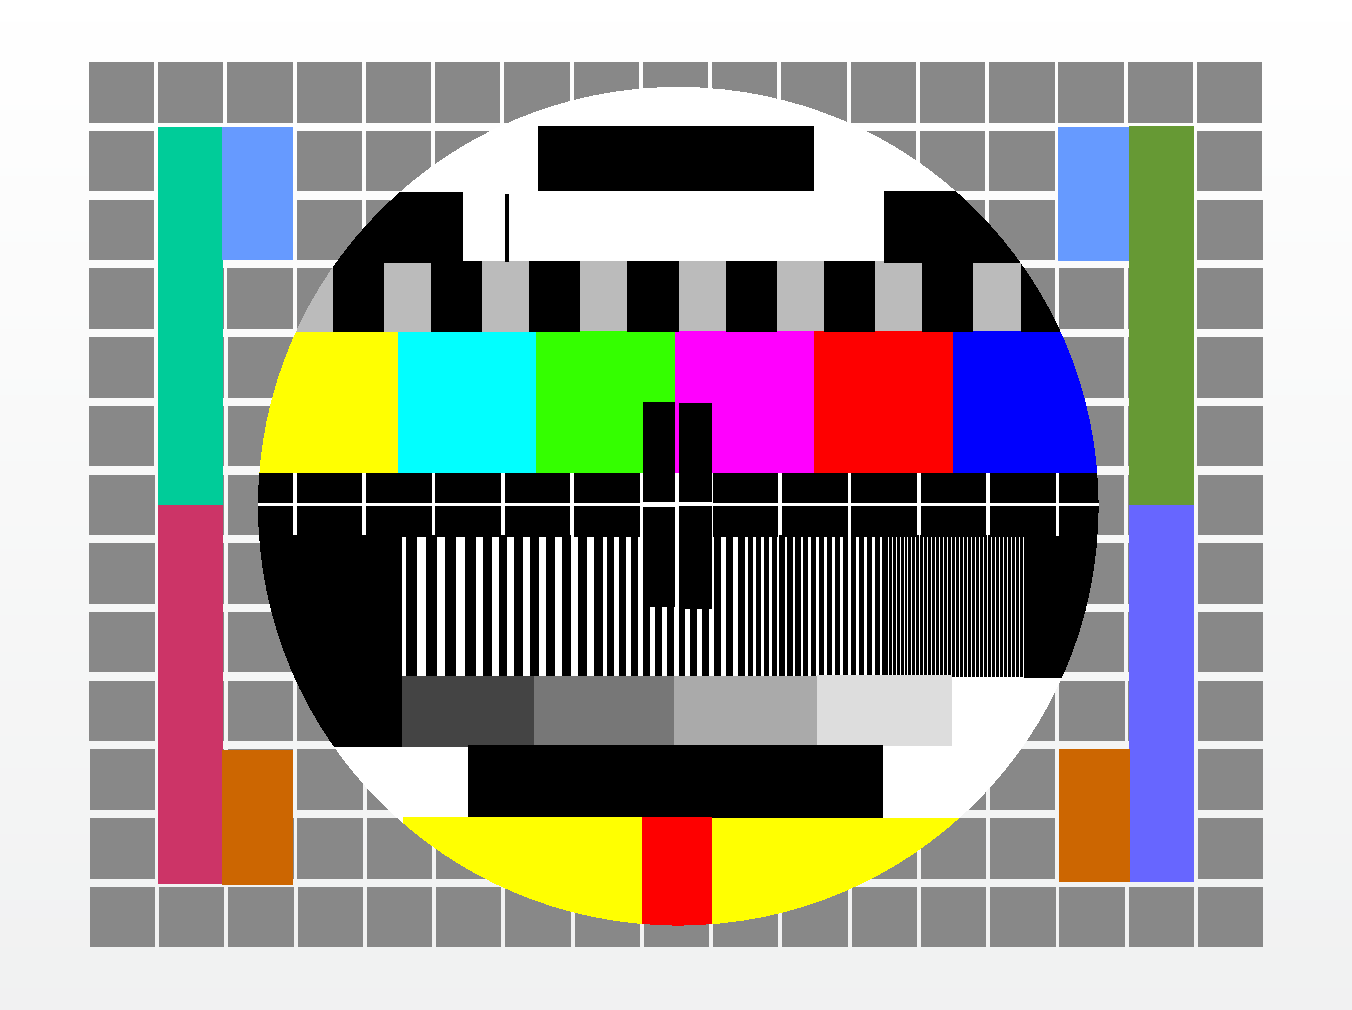
\includegraphics[width=2.5in]{myfigure}
% where an .eps filename suffix will be assumed under latex,
% and a .pdf suffix will be assumed for pdflatex; or what has been declared
% via \DeclareGraphicsExtensions.
\caption{Example of a figure caption.}
\label{fig:example}
\end{figure}

% Note that IEEE typically puts floats only at the top, even when this
% results in a large percentage of a column being occupied by floats.


% An example of a double column floating figure using two subfigures.
% (The subfig.sty package must be loaded for this to work.)
% The subfigure \label commands are set within each subfloat command, the
% \label for the overall figure must come after \caption.
% \hfil must be used as a separator to get equal spacing.
% The subfigure.sty package works much the same way, except \subfigure is
% used instead of \subfloat.
%
%\begin{figure*}[!t]
%\centerline{\subfloat[Case I]\includegraphics[width=2.5in]{subfigcase1}%
%\label{fig_first_case}}
%\hfil
%\subfloat[Case II]{\includegraphics[width=2.5in]{subfigcase2}%
%\label{fig_second_case}}}
%\caption{Simulation results}
%\label{fig_sim}
%\end{figure*}
%
% Note that often IEEE papers with subfigures do not employ subfigure
% captions (using the optional argument to \subfloat), but instead will
% reference/describe all of them (a), (b), etc., within the main caption.


% An example of a floating table. Note that, for IEEE style tables, the
% \caption command should come BEFORE the table. Table text will default to
% \footnotesize as IEEE normally uses this smaller font for tables.
% The \label must come after \caption as always.
%
%\begin{table}[!t]
%% increase table row spacing, adjust to taste
%\renewcommand{\arraystretch}{1.3}
% if using array.sty, it might be a good idea to tweak the value of
% \extrarowheight as needed to properly center the text within the cells
%\caption{An Example of a Table}
%\label{table_example}
%\centering
%% Some packages, such as MDW tools, offer better commands for making tables
%% than the plain LaTeX2e tabular which is used here.
%\begin{tabular}{|c||c|}
%\hline
%One & Two\\
%\hline
%Three & Four\\
%\hline
%\end{tabular}
%\end{table}


% Note that IEEE does not put floats in the very first column - or typically
% anywhere on the first page for that matter. Also, in-text middle ("here")
% positioning is not used. Most IEEE journals/conferences use top floats
% exclusively. Note that, LaTeX2e, unlike IEEE journals/conferences, places
% footnotes above bottom floats. This can be corrected via the \fnbelowfloat
% command of the stfloats package.



% use section* for acknowledgement
\section*{Acknowledgment}

The preferred spelling of the word ``acknowledgment" in America is without an ``e" after the ``g". Avoid the stilted expression, ``One of us (R.B.G.) thanks\ldots". Instead, try ``R.B.G. thanks\ldots". Put sponsor acknowledgments in the unnumbered footnote on the first page.

The following is an example of an acknowledgment.

The authors gratefully acknowledge the contributions of T. Edison, G. Westinghouse, N. Tesla, A. Volta and A. Ampere to the electric power industry.

% trigger a \newpage just before the given reference
% number - used to balance the columns on the last page
% adjust value as needed - may need to be readjusted if
% the document is modified later
%\IEEEtriggeratref{8}
% The "triggered" command can be changed if desired:
%\IEEEtriggercmd{\enlargethispage{-5in}}

% References section
\section*{The References Section}
References are important to the reader; therefore, each citation must be complete and correct. There is no editorial check on references; therefore, an incomplete or wrong reference will be published unless caught by a reviewer and will detract from the authority and value of the paper. References should be readily available publications.

List only one reference per reference number. If a reference is available from two sources, each should be listed as a separate reference.

The template will number citations consecutively within brackets \cite{Fuller1988}. The sentence punctuation follows the bracket \cite{Vidmar1992}. Multiple references \cite{Clarke1950,Young1964} are each numbered with separate brackets \cite{Young1964,Jones1991,Reber1968}. Refer simply to the reference number, as in \cite{Talleen1996}\textemdash do not use ``Ref. \cite{Talleen1996}" or ``reference \cite{Talleen1996}" except at the beginning of a sentence: ``Reference \cite{Talleen1996} was the first\ldots".

Unless there are six authors or more give all authors' names; do not use ``et al.". Papers that have not been published, even if they have been submitted for publication, should be cited as ``unpublished" \cite{Ebehard1984,ProcessCorp,Lester2008}. Capitalize only the first word in a paper title, except for proper nouns and element symbols. For papers published in translation journals, please give the English citation first, followed by the original foreign-language citation \cite{Yorozu}. Papers that have been accepted for publication, but not yet published, should be cited as ``in press'' \cite{Miller}.

Samples of the correct formats for various types of references are given below \cite{Fuller1988,Vidmar1992,Clarke1950,Young1964,Jones1991,Reber1968,Talleen1996,Ebehard1984,ProcessCorp,Lester2008,Yorozu,Miller,Alqueres1991,Hwang1997,IEEE1036-2010,Brandli1978}.

% can use a bibliography generated by BibTeX as a .bbl file
% BibTeX documentation can be easily obtained at:
% http://www.ctan.org/tex-archive/biblio/bibtex/contrib/doc/
% The IEEEtran BibTeX style support page is at:
% http://www.michaelshell.org/tex/ieeetran/bibtex/
%\bibliographystyle{IEEEtran}
% argument is your BibTeX string definitions and bibliography database(s)
%\bibliography{IEEEabrv,../bib/paper}
%
% <OR> manually copy in the resultant .bbl file
% set second argument of \begin to the number of references
% (used to reserve space for the reference number labels box)
\begin{thebibliography}{16}

%Periodicals
\bibitem{Fuller1988}
J.~F.~Fuller, E.~F.~Fuchs, and K.~J.~Roesler, ``Influence of harmonics on power distribution system protection," \emph{IEEE Trans. Power Delivery}, vol. 3, pp. 549-557, Apr. 1988.

\bibitem{Vidmar1992}
R.~J.~Vidmar. (1992, Aug.). On the use of atmospheric plasmas as electromagnetic reflectors. \emph{IEEE Trans. Plasma Sci.} [Online]. \emph{21(3)}, pp. 876-880. Available: \url{http://www.halcyon.com/pub/journals/21ps03-vidmar}

%Books:
\bibitem{Clarke1950}
E. Clarke, \emph{Circuit Analysis of AC Power Systems}, vol. I.  New York: Wiley, 1950, p. 81.

\bibitem{Young1964}
G. O. Young, ``Synthetic structure of industrial plastics," in \emph{Plastics}, 2nd ed., vol. 3, J. Peters, Ed.  New York: McGraw-Hill, 1964, pp. 15-64.

\bibitem{Jones1991}
J. Jones. (1991, May 10). \emph{Networks}. (2nd ed.) [Online]. Available: \url{http://www.atm.com}

%Technical Reports:
\bibitem{Reber1968}
E. E. Reber, R. L. Mitchell, and C. J. Carter, ``Oxygen absorption in the Earth's atmosphere," Aerospace Corp., Los Angeles, CA, Tech. Rep. TR-0200 (4230-46)-3, Nov. 1968.

\bibitem{Talleen1996}
S. L. Talleen. (1996, Apr.). The Intranet Architecture: Managing information in the new paradigm. Amdahl Corp., Sunnyvale, CA. [Online]. Available: \url{http://www.amdahl.com/doc/products/bsg/intra/ infra/html}

%Unpublished Papers:
\bibitem{Ebehard1984}
D. Ebehard and E. Voges, ``Digital single sideband detection for interferometric sensors," unpublished, presented at the 2nd Int. Conf. Optical Fiber Sensors, Stuttgart, Germany, 1984.

\bibitem{ProcessCorp}
Process Corp., Framingham, MA. ``Intranets: Internet technologies deployed behind the firewall for corporate productivity," unpublished. Presented at INET96 Annu. Meeting. [Online]. Available: \url{http://home.process.com/ Intranets/wp2.htp}

\bibitem{Lester2008}
G. N. Lester and J. H. Nelson, ``History of Circuit Breaker Standards," unpublished.  \emph{Presented at the IEEE/PES General Meeting}, 24 July 2008. [Online]. Available IEEE/PES Switchgear Committee web site: \url{http://www.ewh.ieee.org/soc/pes/switchgear/Presentations/2008CBtutorial/speaker1paper.pdf}

%Papers Published in Translation Journals:
\bibitem{Yorozu}
Y. Yorozu, M. Hirano, K. Oka, and Y. Tagawa, ``Electron spectroscopy studies on magneto-optical media and plastic substrate interface," IEEE Transl. J. Magn. Japan, vol. 2, pp. 740–741, August 1987 [Digests 9th Annual Conf. Magnetics Japan, p. 301, 1982].

%Papers Accepted for Publication (but not yet published):
\bibitem{Miller}
E. H. Miller, ``A note on reflector arrays," \emph{IEEE Trans. Antennas Propagat.}, in press.

%Papers from Conference Proceedings (Published):
\bibitem{Alqueres1991}
J. L. Alqueres and J. C. Praca, ``The Brazilian power system and the challenge of the Amazon transmission," in \emph{Proc. 1991 IEEE Power Engineering Society Transmission and Distribution Conf.}, pp. 315-320.

%Dissertations:
\bibitem{Hwang1997}
S. Hwang, ``Frequency domain system identification of helicopter rotor dynamics incorporating models with time periodic coefficients," Ph.D. dissertation, Dept. Aerosp. Eng., Univ. Maryland, College Park, 1997.

%Standards:
\bibitem{IEEE1036-2010}
\emph{IEEE Guide for Application of Shunt Power Capacitors}, IEEE Std. 1036-2010, Sep. 2010.

%Patents:
\bibitem{Brandli1978}
G. Brandli and M. Dick, "Alternating current fed power supply," U.S. Patent 4 084 217, Nov. 4, 1978.


\end{thebibliography}




% that's all folks
\end{document}


